\documentclass[t]{beamer}
\usepackage{listings}
\usepackage{graphicx}
%\tcbset{
%texexp/.style={
%fonttitle=\small\sffamily\bfseries, fontupper=\small, fontlower=\small},
%example/.code 2 args={\refstepcounter{texexp}\label{#2}%
%    \pgfkeysalso{texexp,title={Listing \thetexexp: #1}}},
%}

%Define Colors
\definecolor{gray}{RGB}{102,102,102}		%#666666
\definecolor{lightblue}{RGB}{0,102,153}		%#006699
\definecolor{lightgreen}{RGB}{102,153,0}	%#669900
\definecolor{bluegreen}{RGB}{51,153,126}	%#33997e
\definecolor{magenta}{RGB}{217,74,122}		%#d94a7a
\definecolor{orange}{RGB}{226,102,26}		%#e2661a
\definecolor{purple}{RGB}{181, 0, 209}		%#7d4793
\definecolor{green}{RGB}{113,138,98}		%#718a62

% solarized https://en.wikipedia.org/wiki/Solarized
\definecolor{sblue}{RGB}{38,139,210}
\definecolor{syellow}{RGB}{181,137,0}
\definecolor{sgreen}{RGB}{113,163,0}
\definecolor{sviolet}{RGB}{108,113,196}


\lstdefinelanguage{ispc}{
  %Types
  morekeywords = [1]{int16, int32, int64, uint, uint16, uint32, uint64, int8, uint8, void, int, float, double, float16, int64\_t, int32\_t, char, uint32\_t, memblock, futhark\_context, free\_struct, fs\_struct, mem\_struct, my\_struct *},
  %Control flow
  morekeywords = [2]{catch, do, for, if, else, switch, while, foreach, foreach\_active, cif, return},
  %Qualifiers and stuff
  morekeywords = [3]{uniform, varying, export, extern, struct, unmasked, static, inline, unsigned},
  % Remaining functions
  morekeywords = [4]{extract, insert, reduce\_add, programIndex, programCount, reduce\_op, bin\_op, scan\_op, map\_op},
  keywordstyle = [1]\color{syellow}\bfseries,
  keywordstyle = [2]\color{sgreen}\bfseries,
  keywordstyle = [3]\color{sblue}\bfseries,
  keywordstyle = [4]\color{sviolet}\bfseries,
  sensitive = true,
  morecomment = [l]{//},
  morecomment = [s]{/*}{*/},
  morecomment = [s]{/**}{*/},
  commentstyle = \color{gray},
  morestring = [b]",
  morestring = [b]',
  stringstyle = \color{orange}
}

\lstdefinelanguage{futhark}{
  %Types
  morekeywords = [1]{f32, f64, i32, i64, void, int, float, double, float16, int64\_t, int32\_t, char, uint32\_t, memblock, futhark\_context, free\_struct, fs\_struct, mem\_struct, my\_struct *},
  %Control flow
  morekeywords = [2]{loop, let, def, catch, do, for, if, else, switch, while, foreach, foreach\_active, cif, return},
  %Qualifiers and stuff
  morekeywords = [3]{map, scan, reduce, reduce_by_index, uniform, varying, export, extern, struct, unmasked, static, inline, unsigned},
  % Remaining functions
  morekeywords = [4]{extract, insert, reduce\_add, programIndex, programCount, reduce\_op, bin\_op, scan\_op, map\_op},
  keywordstyle = [1]\color{syellow}\bfseries,
  keywordstyle = [2]\color{sgreen}\bfseries,
  keywordstyle = [3]\color{sblue}\bfseries,
  keywordstyle = [4]\color{sviolet}\bfseries,
  sensitive = true,
  morecomment = [l]{//},
  morecomment = [l]{--},
  morecomment = [s]{/*}{*/},
  morecomment = [s]{/**}{*/},
  commentstyle = \color{gray},
  morestring = [b]",
  morestring = [b]',
  stringstyle = \color{orange}
}

\usepackage{courier}

\lstset{
  basicstyle={\ttfamily\footnotesize},
  identifierstyle={\ttfamily},
  commentstyle={\itshape\ttfamily},
  keywordstyle={\bfseries},
  ndkeywordstyle={\bfseries},
  stringstyle={\ttfamily},
  breaklines=true,
  %columns=[l]{fullflexible},
  xrightmargin=0em,
  xleftmargin=2mm,
  numberstyle={\scriptsize},
  stepnumber=1,
  numbersep=1em,
  lineskip=-0.5ex,
  tabsize=4
}


\usetheme{Madrid}
\usecolortheme{beaver}

\title{Bachelor forsvar}
\subtitle{En ISPC bagende til Futhark}
\author{Kristoffer A. Kortbaek}
\date{23. juni 2022}

%%Front page
\begin{document}
\begin{frame}
  \titlepage
\end{frame}

\begin{frame}[c]
  \frametitle{Fokuspunkt}

  \begin{enumerate}
    \item<+-> Multicore ``flattening''
    \item<+-> Udnyttelse af data parallelisme for \texttt{reduce}
    \item<+-> Hvordan påvirker multicore flattening de data parallelle SOACs
  \end{enumerate}
\end{frame}

%% Slide 1
\begin{frame}[fragile]
  \frametitle{Multicore flattening - sekventielle og parallelle SOACs}
  \begin{onlyenv}<+->
    Et Futhark matrix-vector multiplication program kunne skrives som
\begin{lstlisting}[language=futhark]
    def main m n  (X:[m][n]i32)  (v:[n]i32)  =
      map (\x ->
        reduce (+) 0 (map2 (*) x v)
      ) X
\end{lstlisting}
  \end{onlyenv}
  \only{Hver og bemærke ved programmet}<+->
  \begin{enumerate}
    \item<+-> To parallel SOACs
    \item<+-> En ydre parallel \texttt{map}
    \item<+-> En \textit{nested} \texttt{reduce}
  \end{enumerate}

  \only{Hvordan kan vi afvikle det parallelt på en CPU?}<+->
  \begin{itemize}
    \item<+-> Multicore bagenden kan vælge to metode
  \end{itemize}
   % Programmet har ``nested'' parallelisme grundet den indre \texttt{reduce}
%   \begin{enumerate}
%     \begin{onlyenv}<2-2>
%     \item Hver indre SOAC er blevet sekventialiseret
% \begin{lstlisting}[language=ispc, xleftmargin=-15mm]
%       parfor(i = 0; i < n_cores; i++) {
%         for(int map_i = 0; i < m; map_i++) {
%           int red_res = 0; //Neutral element
%           for(int red_i = 0;  red_i < n; red_i++) {
%             int x = mem[map_i * n + red_i];
%             int v_i = mem[red_i];
%             int mul_res = x * v_i;
%             red_res = mulres + red_res;
%           }
%           mem[map_i] = red_res;
%         }
%       }
% \end{lstlisting}
%   \end{onlyenv}
%     \begin{onlyenv}<3-3>
%     \item De indre SOACs er uberørte og kører i parallel på flere kerner
%       \begin{lstlisting}[language=ispc, xleftmargin=-15mm]
%       parfor() {
%         for(int map_i = 0; i < m; map_i++) {
%           // schedule work for the nested reduce
%           mem[map_i] = reduce_res;
%         }
%       }
%       parfor{
%         for(int red_i = 0;  red_i < n; red_i++) {
%           int x = mem[map_i * n + red_i];
%           int v_i = mem[red_i];
%           int mul_res = x * v_i;
%           red_res = mulres + red_res;
%         }
%       }
%       \end{lstlisting}
%       \end{onlyenv}
%   \end{enumerate}
%   \begin{enumerate}
%     \item<4-> Hvis $m < n_{cores}$ så er der ikke nok arbejde til at ``mætte'' alle CPU kerner. Dette bruges som heuristik for at vælge mellem de to versioner.
    %Hvis den ydre \texttt{map} indeholder flere iterationer end antal logiske kerner på CPUen sekventialiseres \texttt{reduce}
\end{frame}

\begin{frame}[fragile]
  \frametitle{Multicore flattening - sekventielle og parallelle SOACs}
  \begin{onlyenv}<+->
    Kør \texttt{map} parallelt, og den indre \texttt{reduce} kan blive scheduleret ud til ledige tråde
\begin{lstlisting}[language=ispc, xleftmargin=-15mm]
       parfor{
         for(int map_i = 0; i < m; map_i++) {
           // schedule work for the nested reduce
           mem[map_i] = reduce_res;
         }
       }
       parfor{
         for(int red_i = 0;  red_i < n; red_i++) {
           int x = mem[map_i * n + red_i];
           int v_i = mem[red_i];
           int mul_res = x * v_i;
           red_res = mulres + red_res;
         }
       }
\end{lstlisting}
  \end{onlyenv}
  \begin{onlyenv}<+->
    CPU har forholdsvist få kerner
    \begin{itemize}
      \item<+-> Hvad hvis \texttt{map} indeholdte flere iterationer end antal logiske kerner?
      \item<+-> Brug dette som optimisation til at lave ``flattening''
    \end{itemize}
  \end{onlyenv}
\end{frame}

\begin{frame}[fragile]
  \frametitle{Multicore flattening - sekventielle og parallelle SOACs}
  \begin{onlyenv}<+->
    Man kan kører kun selve \texttt{map} i parallel på alle de logiske kerner, og lade \texttt{reduce} blive sekvententialiseret
\begin{lstlisting}[language=ispc, xleftmargin=-15mm]
       parfor(i = 0; i < n_cores; i++) {
         for(int map_i = 0; i < m; map_i++) {
           int red_res = 0; //Neutral element
           for(int red_i = 0;  red_i < n; red_i++) {
             int x = mem[map_i * n + red_i];
             int v_i = mem[red_i];
             int mul_res = x * v_i;
             red_res = mulres + red_res;
           }
           mem[map_i] = red_res;
         }
       }
\end{lstlisting}
  \end{onlyenv}
  \only{Hvis $ n_{cores} < m$, så bliver alle CPU kerner mættede}<+->
\end{frame}
% \begin{frame}
% MC IR indeholder to versioner af hver SOAC
%   \frametitle{Multicore flattening background}
%   \begin{figure}[H]
%     \centering
%     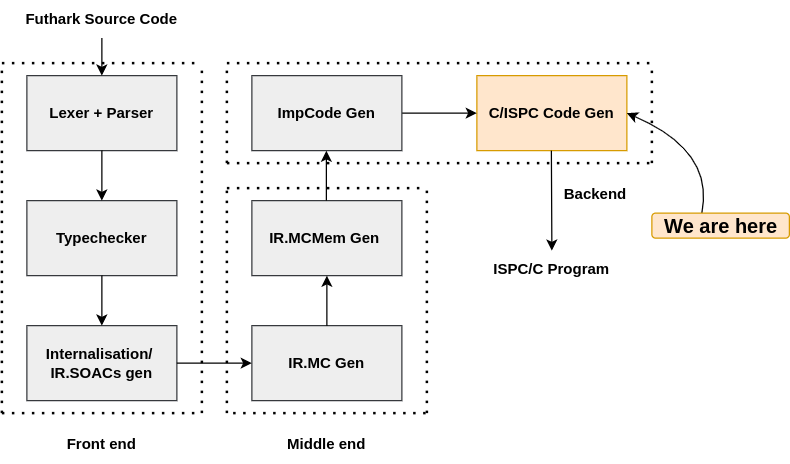
\includegraphics[height=0.7\textheight]{imgs/compileroverview.png}
%   \end{figure}
% \end{frame}

\begin{frame}
  \frametitle{Multicore flattening - sekventielle og parallelle SOACs}
  \only{De to versioner bruges af multicore bagenden, og bliver valgt på runtime}<+->
  \begin{enumerate}
    \item<+-> Den flattenede/sekventialiserede version vælges hvis der er nok iterationer på den yderste SOAC til at mætte CPU kernerne
    \item<+-> Den uberørte parallelle version vælges ellers.
  \end{enumerate}
  \only{Kan vi finde mere parallelisme?}<+->
  \begin{itemize}
    \item<+-> Udnyttelse af SIMD indenfor hver tråd
  \end{itemize}
\end{frame}

\begin{frame}[fragile]
  \frametitle{Udvidelse af multicore flattening}
  \only{Brug ISPC til at udvide både de sekventielle og nestede SOACs}<+->
  \begin{enumerate}
    \item<+-> Hver tråds arbejde skal køre i ISPC - en såkaldt \textit{ISPC kernel}
    \item<+-> Benyt \texttt{foreach} hvor muligt
  \end{enumerate}
  \only{Vi prøvede forskellige måde at udnytte  language-c-quote til at generere selve ISPC koden}<+->
  \begin{enumerate}
    \item<+-> Generer C kode og misbrug makroer til at lave ISPC kode
          %override c keywords - qualifiersJJ
\begin{lstlisting}[language=ispc, xleftmargin=-20mm]
            #define auto uniform
            auto int foo = free->foo;
          \end{lstlisting}
    \item<+-> Udvid language-c-quote med ISPC sprog konstruktioner
          \begin{lstlisting}[xleftmargin=-20mm]
            [C.cstm|foreach ($foreachiters:bounds) {$items:body}|]
          \end{lstlisting}
    \item<+-> Brug ecaped statements
          \begin{lstlisting}[xleftmargin=-20mm]
            [C.cstms|$escstm:("foreach (i=0 ... end)") { $items:body}|]
          \end{lstlisting}
  \end{enumerate}


\end{frame}

%% Slide 2

\begin{frame}
  \frametitle{Algoritmer til at udvide Futhark MC flattening}
  Hvordan kan man vektorisere de to forskellige versioner af en SOAC?
  \begin{enumerate}
    %\item Vores kodegenerator er ``dum'' omkring hvorvidt vi laver kode for en nested eller sekventialiseret SOAC
  % \item Begge versioner af en given SOAC kan tage gavn af data parallelisme
  % \item Vi udnytter et ekstra lag af parallelisme ved at lade hver tråd udnytte data parallelisme
  \item<+-> Giv hver SOAC en specifik vectoriseret algoritme afhængigt af operatoren
  \item<+-> Håndter scheduling fra ISPC
  \item<+-> Særligt har redomap fire forskellige kodegenereringer
    \begin{itemize}
    \item<+-> kommutative \texttt{reduce}
    \item<.> normal(ikke kommutative) \texttt{reduce}
    \item<.> \texttt{reduce} på en ``mapped'' operator
    \item<.> Ingen brug af vektorisering
    \end{itemize}
  \end{enumerate}
\end{frame}

\begin{frame}[fragile]
  \frametitle{Kommutative reduktioner}
  \begin{block}{Kommutative Reduktioner genereres der særligt effektiv kode for}
  \begin{enumerate}
    \item Den binære operator kan ske i vilkårlig rækkefølge: $a + b = b + a$
          %Nævn at i vores rapport kalder vi det interleaved
    \item Hver \textit{program instance} kan arbejde på sit eget segment af inputtet
  \end{enumerate}
\end{block}
\begin{onlyenv}<+->
  Simple reduktion over input array
  \begin{columns}
  \column{0.49\textwidth}
  \begin{figure}[H]
  \centering
  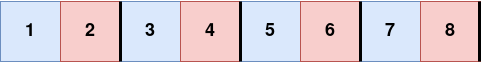
\includegraphics[width=0.9\textwidth]{imgs/input.png}
\end{figure}
\column{0.49\textwidth}

  \begin{lstlisting}[language=futhark]
    reduce (+) 0 as
  \end{lstlisting}

\end{columns}
\end{onlyenv}
\begin{onlyenv}<+->
  Den vectoriserede algoritme for kommutative \texttt{redomap}s har 2 skridt
  \begin{figure}[h!]
    \centering
    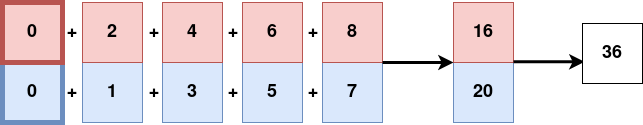
\includegraphics[width=0.7\textwidth]{imgs/kom_reduction.png}
  \end{figure}
\end{onlyenv}
\end{frame}
\begin{frame}[fragile]
  \frametitle{Kommutativ reduction 1}
  Hver program instance laver sin egen reduktion.
\begin{lstlisting}[language=ispc]
    int acc = 0;
    uniform int uni_acc = 0;
    foreach(Reduce_i = 0 ... n) {
      int a = mem[Reduce_i];
      int res = acc + a;
      acc = res;
    }
\end{lstlisting}
  \begin{figure}[H]
    \centering
    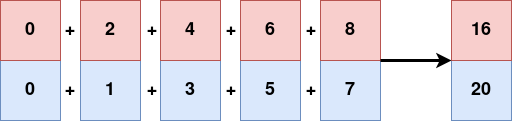
\includegraphics[width=0.5\textwidth]{imgs/kom_reduce1.png}
  \end{figure}
  \begin{center}
  \end{center}
\end{frame}
\begin{frame}[fragile]
  \frametitle{Kommutativ reduction 2}
  Derefter reduceres over resultaterne produceret af et \textit{gang}
  \begin{lstlisting}[language=ispc]
    forneach_active{i = 0 ... programCount} {
      uniform int a = extract(acc, i);
      uniformint res = uni_acc + a
      uni_acc = res;
    }
    mem_out[out] = uni_acc;
\end{lstlisting}
  \begin{figure}[H]
    \centering
    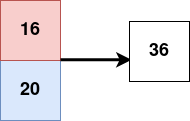
\includegraphics[width=0.25\textwidth]{imgs/kom_reduce2.png}
  \end{figure}
  %Nævn der ikke er en garanti for rækkefølgen af program instansernes operatioenr
\end{frame}

\begin{frame}
  \frametitle{Kommutativ reduktion restriktion}
  Vi har yderst god udnyttelse af SIMD
  \begin{enumerate}
    \item<+-> Hver program instance kører hele tiden
  \end{enumerate}
  \only{Vi kan dog se at der ikke er garanti for rækkefølgen af reduktionen}<+->
  \begin{enumerate}
    \item<+-> Den ene program instance regner $2+4+6+8$
    \item<+-> Den anden regner $1+3+5+7$
  \end{enumerate}
  \only{Derved bliver vi nødt til at håndtere generelle associative operatorer anderledes}<+>
\end{frame}

\begin{frame}[fragile]
  \frametitle{Associative redomap}
  \begin{onlyenv}<+->
    \begin{block}{Associative reduktioner leder til delvis SIMD udnyttelse}
      \begin{enumerate}
        \item Den binære operator skal påføres i specifik rækkefølge
        \item Vi kan ikke lade hver \textit{program instance} arbejde på sit eget segment
        \item Mapping functionen bliver vektoriseret og selve \texttt{reduce} kører sekventielt
      \end{enumerate}
    \end{block}
  \end{onlyenv}
  \begin{onlyenv}<+->
    Vi håndterer korrekt nested parallelisme og sekventialiserede SOACs ved at \textit{sekventialisere} selve \texttt{reduce} operatoren
\begin{lstlisting}[language=ispc]
    uniform int scalar_accum = neutral;
    foreach (i = 0 ... size) {
      int elem_i = arr[i];
      int mapped = map_op(elem_i);
      foreach_active (j) {
        uniform int elem_j = extract(mapped, j);
        scalar_accum = reduce_op(scalar_accum, elem_j); }
    }
    return scalar_accum;
\end{lstlisting}
  \end{onlyenv}
\end{frame}

\begin{frame}[fragile]
  \frametitle{Redomap på en \textit{mapped} operator}
  \begin{onlyenv}<+->
    \begin{block}{Mapped operator}
      \begin{enumerate}
        \item Kan være en \texttt{reduce} eller \texttt{scan} med en \texttt{map2} som operator
        \item Særtilfælde hvor operatoren er på arrays, og vi generer ISPC kode
      \end{enumerate}
    \end{block}
  \end{onlyenv}
  % \begin{block}{Mapped operator er et særtilfælde af der handles effektivt}
  %   \begin{enumerate}
  %   \item Særtilfælde der kan håndterer operatorer der tager arrays
  %   \item Håndteres ofte effektivit da vi kan vektorisere den indre operator
  %   \end{enumerate}
  % \end{block}
  \begin{onlyenv}<+->
    Simpelt program der tager en \textit{mapped} operator i form af \texttt{map2}
\begin{lstlisting}[language=futhark]
  entry mapped_plus [m][n] (X: [m][n]f32) =
    let a = replicate n 0
    in reduce (map2 (+)) a X

\end{lstlisting}
  \end{onlyenv}
\end{frame}

\begin{frame}[fragile]
  \frametitle{Redomap \textit{mapped} operator eksempel}
  \begin{center}
  \only<+>{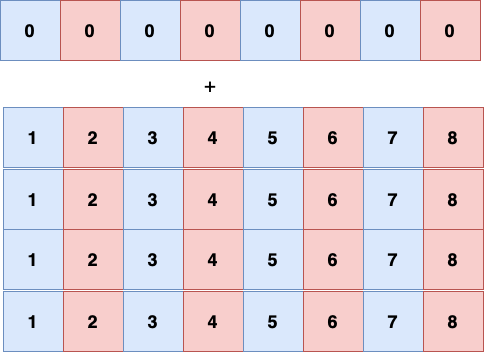
\includegraphics[width=0.7\textwidth]{imgs/mapped1}}
  \only<+>{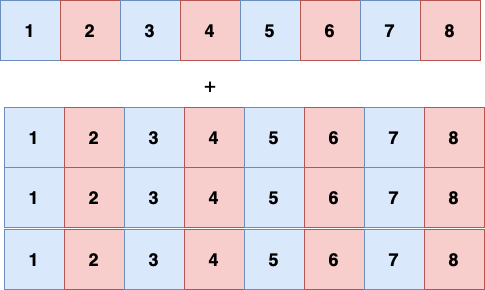
\includegraphics[width=0.7\textwidth]{imgs/mapped2}}
  \only<+>{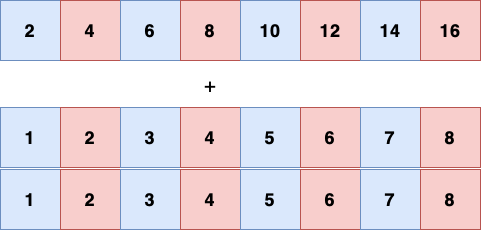
\includegraphics[width=0.7\textwidth]{imgs/mapped3}}
  \only<+>{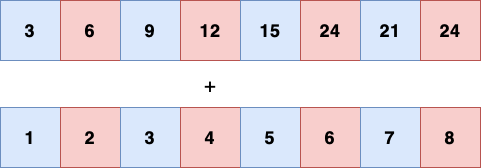
\includegraphics[width=0.7\textwidth]{imgs/mapped4}}
  \only<+>{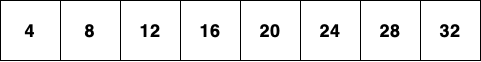
\includegraphics[width=0.7\textwidth]{imgs/mapped5}}
  \end{center}
\end{frame}

\begin{frame}[fragile]
  \frametitle{Redomap \textit{mapped} operator algoritme}
  Observationer
  \begin{enumerate}
    \item<+-> Applikationen af $+$ er uafhængig af \texttt{map2} loop iterationer
    \item<+-> Istedet kører $+$ ``på tværs'' af hvert \texttt{reduce} loop iterationer
    \item<+-> Vi kan derved sikkert vektorisere selve $+$ operatoren
  \end{enumerate}
  \begin{onlyenv}<+->
    \begin{block}{redomap med en mapped operator}
\begin{lstlisting}[language=ispc]
      uniform int acc_mem[m] = //some memory
      for(uniform int red_i = 0; scan_i < i; sca_i++) {
        foreach(nest_i = 0 ... m) {
          x_acc = acc_mem[nest_i];
          x = mem[red_i * n + nest_i];
          int res = x_acc + x;
          acc_mem[nest_i] = res;
        }
      }
\end{lstlisting}
    \end{block}
  \end{onlyenv}
  \end{frame}

%% Slide 3
\begin{frame}[fragile]
  \frametitle{Kombinering af MC flattening og vektoriserede algoritmer}
  \only{Er vores algoritmer en god udvidelse af MC flattening?}<+->
  \begin{enumerate}
    \item<+-> Sekventialiserede SOACs giver oftte \textit{scatter} og \textit{gather} operationer\\
      \begin{onlyenv}<+-3>
        Matrix vector multiplication programmet
        \begin{lstlisting}[language=futhark]
    def main m n  (X:[m][n]i32)  (v:[n]i32)  =
      map (\x ->
        reduce (+) 0 (map2 (*) x v)
      ) X
\end{lstlisting}
      \end{onlyenv}
      \begin{onlyenv}<3-7>
      \begin{columns}
        \begin{column}{0.49\textwidth}
        \begin{lstlisting}[language=ispc, xleftmargin=-15mm, breaklines=false]
        //Sekventialiseret
        foreach(map_i = 0 ... end) {
          for(uniform int red_i = 0;
              red_i < n; red_i++) {
            x = mem[map_i * n + red_i];
          }
        }
\end{lstlisting}
        \end{column}
        \begin{column}{0.49\textwidth}
        \begin{lstlisting}[language=ispc, xleftmargin=-15mm, breaklines=false]
        //Nested reduce
        uniform map_i; uniform n;
        ...
        foreach(red_i = 0 ... end) {
          x = mem[map_i * n + red_i];
        }
\end{lstlisting}
          \end{column}
        \end{columns}
      \end{onlyenv}
  \begin{onlyenv}<+->
    For alle $n \neq 1$ vil det give en \textit{gather} instruction da memory load ikke vil være \textit{coherent}
  \end{onlyenv}
  \begin{onlyenv}<+>
    $$
    \texttt{map\_i} \cdot n =\left<0, 1, 2, 3 \right> \cdot 2 = \left<0,2,4,6\right>
    $$
  \end{onlyenv}

    \item<+-> Nested parallelisme giver derimod vector loads grundet \textit{coherent} memory access
          \begin{onlyenv}<+>
            $$red\_i=\left<0, 1, 2, 3\right>$$
            \end{onlyenv}

  \begin{onlyenv}<+>
    \begin{table}[H]
      \begin{tabular}{|l|l|l|l|l|}
      \hline
      Benchmark                                                  &  & Multicore (ms) & Ours (ms) & Speedup \\ \cline{1-1} \cline{3-5}
      \begin{tabular}[c]{@{}l@{}}$m=100, n=100000$\end{tabular} &  & 1              & 3         & x0.44   \\ \cline{1-1} \cline{3-5}
      \begin{tabular}[c]{@{}l@{}}$m=6, n=10000000$\end{tabular} &  & 12             & 12        & x0.97   \\ \hline
      \end{tabular}
    \end{table}
  \end{onlyenv}
    \item<+-> Mapped operator giver gode loads/store for sekventialiserede SOACs
      \begin{onlyenv}<+>
        \begin{lstlisting}[language=futhark]
          entry mapped_plus [m][n] (X: [m][n]f32) : [n]f32 =
            let a = replicate n 0
            in reduce (map2 (f32.min)) a X
        \end{lstlisting}
      \end{onlyenv}
      \begin{onlyenv}<+>
       \begin{lstlisting}[language=ispc, xleftmargin=-15mm]
             uniform int acc_mem[m] = //some memory
             for(uniform int red_i = 0; scan_i < i; sca_i++) {
               foreach(nest_i = 0 ... m) {
                 x_acc = acc_mem[nest_i];
                 x = mem[red_i * n + nest_i];
                 int res = x_acc + x;
                 acc_mem[nest_i] = res;
               }
             }
       \end{lstlisting}
      \begin{table}[H]
      \begin{tabular}{|l|l|l|l|l|}
      \hline
      Benchmark                                                  &  & Multicore (ms) & Ours (ms) & Speedup \\ \cline{1-1} \cline{3-5}
      \begin{tabular}[c]{@{}l@{}}$m=100000, n=1000$\end{tabular} &  & 3.6             & 1.1       & x3.23   \\ \cline{1-1} \cline{3-5}
      \begin{tabular}[c]{@{}l@{}}$m=1000, n=100000$\end{tabular} &  & 84             & 81.2        & x1.03   \\ \hline
      \end{tabular}
      \end{table}

    \end{onlyenv}
\end{enumerate}
\end{frame}

  \begin{frame}
    \frametitle{Konklusion}
    \begin{enumerate}
      \item<+-> Vi har på en let måde fået ekstra speedup på multicore bagenden uden at ændre tidligere stadier af compileren
    \item<+-> Identificeret steder hvor vi kan lave forbedringer til compileren, for at gøre memory accesses hurtigere
    \end{enumerate}
  \end{frame}
\end{document}
